\subsubsection{施洗约翰被囚前\href{http://biblegeography.holylight.org.tw/index/condensedbible_map_detail?m_id=108}{(耶稣受洗初期服事路线)}}
\begin{table}[H]
\centering
\begin{tabular}{p{6.45em}|c|p{4.785em}|r|p{3.em}|p{3.23em}|p{3.5em}}\toprule

\multicolumn{2}{p{20.5em}|}{事 件} & 地 點& \multicolumn{1}{p{3.23em}|}{太} & \multicolumn{1}{p{3.23em}|}{可}    & \multicolumn{1}{p{3.23em}|}{路} & \multicolumn{1}{p{3.5em}}{約} \\\midrule\midrule

\multicolumn{2}{p{20.5em}|}{耶穌約三十歲開頭傳道} & \multicolumn{1}{p{5.355em}|}{加利利} &\multicolumn{1}{p{4.145em}|}{}&\multicolumn{1}{p{3.85em}|}{}&\multicolumn{1}{p{3.5em}|}{3:23}& \\ \midrule

\multirow{5}[8]{*}{五門徒跟從耶穌} & \multicolumn{1}{p{13.355em}|}{次日約翰門徒(約翰/安德烈)} & \multirow{4}[8]{*}{約但河} & & && 1:35-39 \\

\cmidrule{2-2}\cmidrule{4-7}    \multicolumn{1}{c|}{} & \multicolumn{1}{p{13.355em}|}{安德烈领西門歸主,改名彼得} & \multicolumn{1}{c|}{} & & & & 1:40-42 \\

\cmidrule{2-2}\cmidrule{4-7}    \multicolumn{1}{c|}{} & \multicolumn{1}{p{13.355em}|}{又次日去加利利路上呼召腓力} & \multicolumn{1}{c|}{} &  & & & 1:43-44 \\

\cmidrule{2-2}\cmidrule{4-7}\multicolumn{1}{c|}{} & \multicolumn{1}{p{13.355em}|}{伯賽大人腓力领拿但業歸主}&\multicolumn{1}{c|}{}&&&&1:45-48\\

\cmidrule{2-2}\cmidrule{4-7}\multicolumn{1}{c|}{} & \multicolumn{1}{p{13.355em}|}{迦拿人拿但業认耶稣为神兒子}&\multicolumn{1}{c|}{}&&&&1:49-51\\\midrule

\multicolumn{2}{p{20.5em}|}{第一個神迹:婚宴變水為酒}&迦拿&&&& 2:1-11\\\midrule

\multicolumn{2}{p{20.5em}|}{耶穌第一次與門徒去迦百農住了不多幾日}&迦百農&&&&2:12\\\midrule

耶穌潔淨聖殿 & 
\multicolumn{1}{c|}{\multirow{3}[6]{*}{第一个逾越節}} &
\multicolumn{1}{l|}{\multirow{3}[6]{*}{耶路撒冷}}&&&&2:13-17\\

\cmidrule{1-1}\cmidrule{4-7}三日再建圣殿&&&&&& 2:18-22 \\
\cmidrule{1-1}\cmidrule{4-7} 行好些神迹 &（共四个逾越节）&&&&& 2:23-25 \\
\cmidrule{1-1}\cmidrule{4-7} 尼哥底母夜访&&&&&&3:1-21\\\midrule

\multicolumn{2}{p{20.5em}|}{耶穌的門徒給人施浸} & \multicolumn{1}{p{5.355em}|}{猶太地} &       &       &       & 3:22\\\midrule

\multicolumn{2}{p{20.5em}|}{施洗\textcolor{red}{約翰}最後的見證:他必興旺我必衰微} & \multicolumn{1}{p{5.355em}|}{撒冷的哀嫩} &       &       &       & 3:23-36 \\ \midrule

\multicolumn{2}{p{20.5em}|}{法利賽人見主施洗比約翰多,耶穌離開猶太地} & \multicolumn{1}{p{5.355em}|}{猶太地} &       &       &       & 4:1-3a\\\midrule

\multicolumn{2}{p{20.5em}|}{耶穌與撒馬利亞婦人谈用心靈和誠實拜父傳道} & 
\multicolumn{1}{l|}{\multirow{2}[6]{*}{敘加}} &       &       &       & 4:3b-30\\

\cmidrule{1-2}\cmidrule{4-7}\multicolumn{2}{p{20.5em}|}{對門徒讲:食物是遵行父的旨意，莊稼熟了} &  &       &       &       & 4:31-38\\ 

\cmidrule{1-2}\cmidrule{4-7}\multicolumn{2}{p{20.5em}|}{福音在敘加傳開} &  &       &       &       & 4:39-42 \\ \midrule

\multicolumn{2}{p{20.5em}|}{加利利人見主在耶京所行的就接待他} & \multicolumn{1}{p{5.355em}|}{迦拿} &       &       &       & 4:43-45 \\ \midrule
\multicolumn{2}{p{20.5em}|}{第二個神迹:在迦拿醫治大臣兒子(在迦百農)} & \multicolumn{1}{p{5.355em}|}{迦拿} &       &       &       & 4:46-54 \\ \midrule
\end{tabular}
\caption{两个神迹/3(耶稣)+1(约翰)讲道}
\end{table}

\begin{figure}[H]
\centering
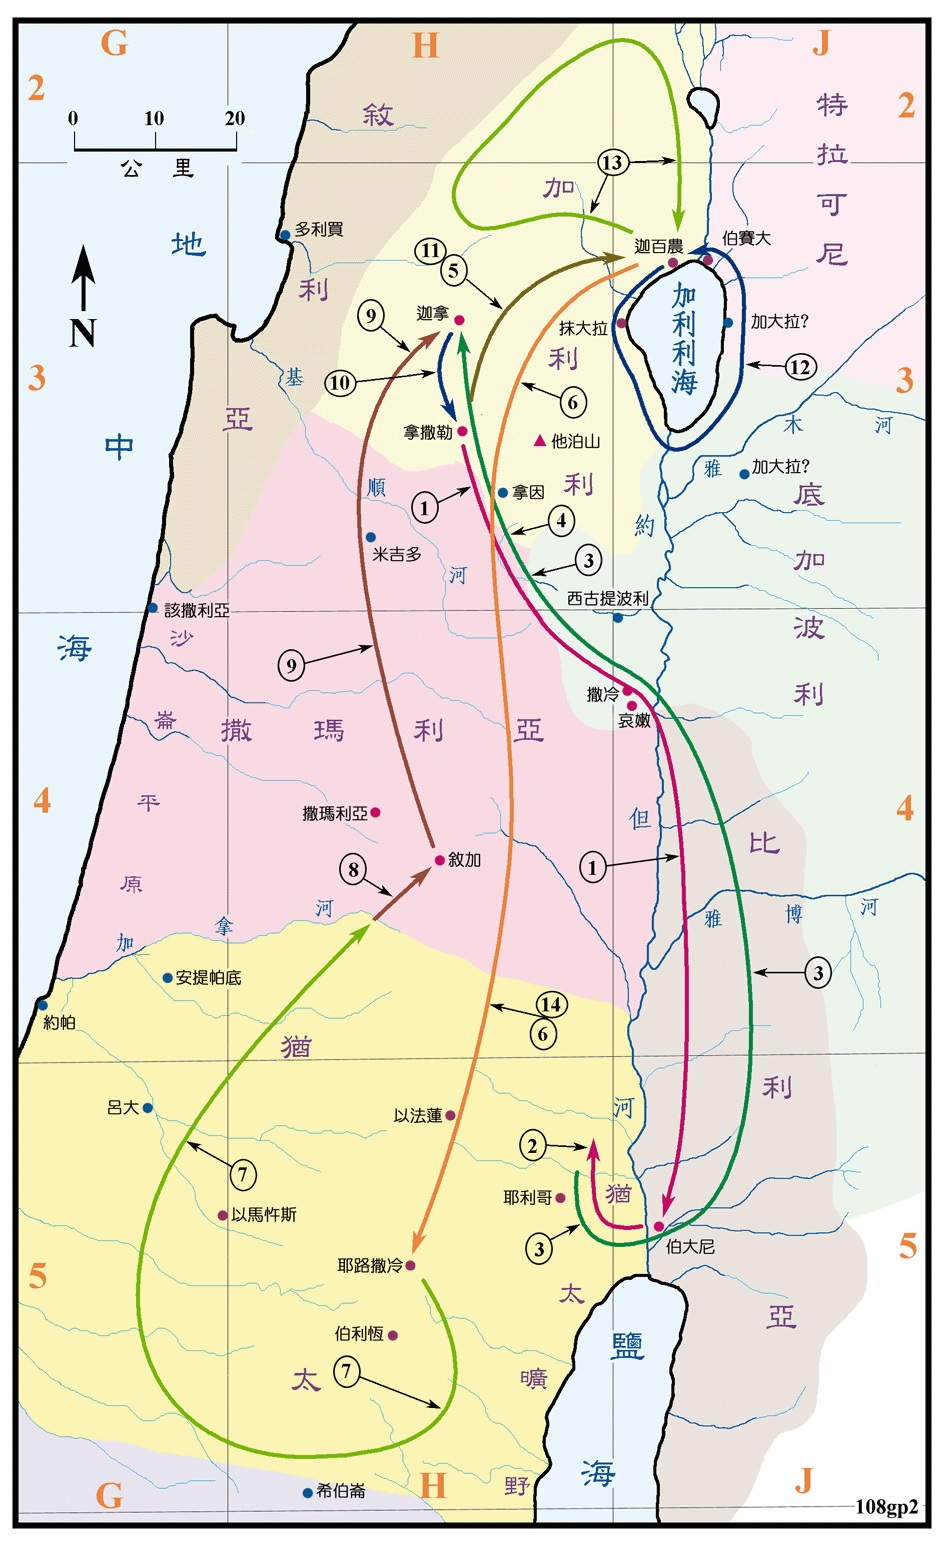
\includegraphics[width=150mm]{ZongJie/SiFuYin/figs/jesustripYouth} 
\caption{初期服事路线}
\end{figure}

\subsubsection{施洗约翰被囚后开始呼召门徒\href{http://biblegeography.holylight.org.tw/index/condensedbible_map_detail?m_id=109}{(揀選门徒后的服事)}}

\begin{table}[H]\centering 
\begin{tabular}{p{6.45em}|c|p{4.785em}|r|p{6.em}|p{3.23em}|p{1.em}}\toprule

\multicolumn{2}{p{20.em}|}{事 件} & 地 點& \multicolumn{1}{p{3.23em}|}{太} & \multicolumn{1}{p{3.23em}|}{可}    & \multicolumn{1}{p{3.23em}|}{路} & \multicolumn{1}{p{1.em}}{約} \\\midrule\midrule

\cmidrule{1-2}\cmidrule{4-7}\multicolumn{2}{p{20.em}|}{安息日在迦百農會堂裡趕逐汙鬼傳道} &\multicolumn{1}{l|}{\multirow{4}{*}{迦百農}}  &  & \multicolumn{1}{p{4.43em}|}{1:21-28} & \multicolumn{1}{p{3.5em}|}{4:31-37} & \multicolumn{1}{r}{} \\ 

\cmidrule{1-2}\cmidrule{4-7}\multicolumn{2}{p{20.em}|}{安息日在西門家醫彼得岳母熱病} && \multicolumn{1}{p{4.145em}|}{8:14-15} & \multicolumn{1}{p{4.43em}|}{1:29-31} & \multicolumn{1}{p{3.5em}|}{4:38-39} & \multicolumn{1}{r}{} \\ 

\cmidrule{1-2}\cmidrule{4-7}\multicolumn{2}{p{20.em}|}{晚上醫治各樣病人,應驗以賽亞预言} && \multicolumn{1}{p{4.145em}|}{8:16-17} & \multicolumn{1}{p{4.43em}|}{1:32-34} & \multicolumn{1}{p{3.5em}|}{4:40-41} &  \\ 


\cmidrule{1-2}\cmidrule{4-7}\multicolumn{2}{p{20.em}|}{湖边二次召彼得/雅各/約翰得人如得鱼} &  & \multicolumn{1}{p{4.145em}|}{} & \multicolumn{1}{p{4.43em}|}{} & \multicolumn{1}{p{3.5em}|}{5:1-11} &\\

\cmidrule{1-2}\cmidrule{4-7}\multicolumn{2}{p{20.5em}|}{山下的城裡伸手摸,醫治長大痲瘋的人} &  & \multicolumn{1}{p{4.145em}|}{8:1-4} & \multicolumn{1}{p{4.43em}|}{1:40-45} & \multicolumn{1}{p{3.5em}|}{5:12-16} & \multicolumn{1}{c}{} \\ \midrule

\multicolumn{2}{p{20.em}|}{在法利賽人和教法師面前醫四人擡癱子} & \multicolumn{1}{l|}{\multirow{5}{*}{迦百農}}& \multicolumn{1}{p{4.145em}|}{9:1-8} & \multicolumn{1}{p{4.43em}|}{2:1-12} & \multicolumn{1}{p{3.5em}|}{5:17-26} & \\


\multicolumn{2}{p{20.em}|}{畢士大池醫38年瘫子} & \multicolumn{1}{l|}{\multirow{5}{*}{耶京(更晚?)}}& &  & &\multicolumn{1}{p{3.95em}}{5:1-15}\\ \midrule


\multicolumn{2}{p{12.em}|}{安息日在會堂醫枯右手者}&\multicolumn{1}{p{7.1em}|}{離開麥地進會堂}&\multicolumn{1}{p{4.em}|}{12:9-13}&\multicolumn{1}{p{4.43em}|}{3:1-5}&\multicolumn{1}{p{4.em}|}{6:6-10}& \\ \midrule

\end{tabular}

\end{table}


